\documentclass{article}

\usepackage{graphicx}
\usepackage{float}
\usepackage{array}
\usepackage{amssymb}
\usepackage{amsmath}
\usepackage{booktabs}


\begin{document}

  \begin{titlepage}
    \centering
    \vspace*{2cm}
    
    \Huge
    \textbf{Simulador de Polarización en Redes}
    
    \vspace{1.5cm}
    
    \Large
    Jhorman Gomez{\textsuperscript{1}}, Ivan Ausecha{\textsuperscript{2}}, James Calero{\textsuperscript{3}}, Daniel Rojas{\textsubscript{4}}
    
    \vspace{0.5cm}
    
    \large

    2326867{\textsuperscript{1}}, -{\textsuperscript{2}}, 2243461{\textsuperscript{3}}, 2040170{\textsuperscript{4}}
   
    
    \vspace{0.5cm}
    
    \Large
    Universidad del Valle
    
    \vspace{0.5cm}
    
    \large
    Facultad de Ingeniería
    
    \vspace{0.5cm}
    
    \large
    Escuela de Ingeniería de Sistemas y Computación
    
    \vspace{0.5cm}
    
    \large
    Santiago de Cali, Noviembre de 2024
    
  \end{titlepage}
\section{Introducción}

\paragraph{}
El presente documento describe el desarrollo y funcionamiento de un \textbf{Simulador de Polarización en Redes}, herramienta que busca modelar y analizar los fenómenos de polarización social utilizando técnicas avanzadas de programación y estructuras de datos. 
\\

El trabajo se centra en el uso de algoritmos basados en funciones de alto orden, colecciones y procesos recursivos, así como en la implementación de paralelismo de datos para optimizar el rendimiento del simulador. Además, se describen las técnicas empleadas en funciones clave, como \textbf{min\_p, rhoCMT\_Gen, rho, confBiasUpdate} y \textbf{simulate}, junto con su impacto en la precisión y eficiencia del modelo.
\\

Por último, se presentan los resultados de las pruebas realizadas, destacando las ventajas del paralelismo de datos frente a otras técnicas y ofreciendo una comparación detallada de su impacto en el desempeño del simulador. Este documento busca servir como una guía técnica y como referencia para futuras implementaciones relacionadas con la simulación de fenómenos sociales.


  \section{¿Son Nuestras Funciones Funcionalmente Puras?}

  \begin{table}[H]
    \centering
    \begin{tabular}{|c|c|p{5cm}|}
    \hline
    \textbf{Función} & \textbf{Funcional} & \textbf{¿Por qué no?} \\ \hline
    min\_p & Si & - \\ \hline
    rhoCMT\_Gen & Si & - \\ \hline
    normalizar & Si & - \\ \hline
    rho & Si & - \\ \hline
    showWeightedGraph & Si & - \\ \hline
    confBiasUpdate & Si & - \\ \hline
    simulate & Si & - \\ \hline
    rhoPar & No & A pesar de que no hay efectos secundarios por el uso de paralelismo, la función no es funcionalmente pura por el no determinismo en el orden de realización de las operaciones dentro de esta. \\ \hline
    confBiasUpdatePar & No & A pesar de que no hay efectos secundarios por el uso de paralelismo, la función no es funcionalmente pura por el no determinismo en el orden de realización de las operaciones dentro de esta. \\ \hline
    \end{tabular}
  \end{table}

  \section{Técnicas y Estructuras de Datos Utilizadas}
    
    \subsection{min\_p}
    La función \textbf{min\_p} hace uso de:

    \begin{itemize}
      \item \textbf{Recursión:} genera un proceso de recursión lineal mediante el cual por cada iteración se aproxima más al punto mínimo de la función recibida.
      \item \textbf{Funciones de Alto Orden:} recibe una función como parámetro.
      \item \textbf{Colecciones:} genera un rango de valores a partir del min y max recibidos, a este rango se le aplica un map y al resultado del map se le aplica el método minBy, ambos métodos pertenecientes a colecciones.
    \end{itemize}

    \subsection{rhoCMT\_Gen}
    La función \textbf{rhoCMT\_Gen} hace uso de:

    \begin{itemize}
      \item \textbf{Funciones de Alto Orden:} hace uso de funciones anónimas y retorna esta misma como resultado.
      \item \textbf{Colecciones:} hace uso del método zip para generar una colección de tuplas (Frecuency, DistributionValue) sobre la cual se define la función sum.
    \end{itemize}

    \subsection{normalizar}
    La función \textbf{normalizar} hace uso de:

    \begin{itemize}
      \item \textbf{Funciones de Alto Orden:} hace uso de funciones anónimas y retorna esta misma como resultado.
      \item \textbf{Colecciones:} hace uso de vectores y en especial el método fill para generar una colección con la mayor polarización posible para una frecuencia de longitud k.
    \end{itemize}

    \subsection{rho}
    La función \textbf{rho} hace uso de:

    \begin{itemize}
      \item \textbf{Funciones de Alto Orden:} hace uso de funciones anónimas y retorna esta misma como resultado.
      \item \textbf{Colecciones:} hace uso de colecciones y métodos característicos de estas para generar los intervalos sobre los cuales se van a clasificar los agentes y a su vez estos se clasifican haciendo uso de métodos como map y groupBy.
      \item \textbf{Iteradores:} hace uso de métodos que requieren de iteradores como ZipWithIndex y indexWhere.
      \item \textbf{Reconocimiento de Patrones:} hace uso de reconocimiento de patrones para el reconocimiento de los elementos que hacen parte de las colecciones utilizadas, esto con el fin de poder hacer transformaciones sobre dichas colecciones y en últimas clasificar los agentes y obtener la frecuencia final a partir de las opiniones de estos.
    \end{itemize}

    \subsection{showWeightedGraph}
    La función \textbf{showWeightedGraph} hace uso de:

    \begin{itemize}
      \item \textbf{Funciones de Alto Orden:} recibe funciones como parámetro, en específico la función swg que corresponderia a la matriz de influencia.
    \end{itemize}

    \subsection{confBiasUpdate}
    La función \textbf{confBiasUpdate} hace uso de:

    \begin{itemize}
      \item \textbf{Funciones de Alto Orden:} recibe funciones como parámetro, en específico la función swg que corresponderia a la matriz de influencia.
      \item \textbf{Colecciones:} recibe una colección y en base a esta mediante el uso de map, se define la función sum sobre la que se va a realizar el respectivo update a las creencias de los agentes haciendo uso de un rango y mapeando dicha función para cada valor del rango.
    \end{itemize}

    \subsection{simulate}
    La función \textbf{simulate} hace uso de:

    \begin{itemize}
      \item \textbf{Funciones de Alto Orden:} recibe funciones como parámetro, en específico las funciones correspondientes a la matriz de influencia (swg) y la función sobre la cual se van a actualizar las creencias de los agentes (fg).
      \item \textbf{Colecciones:} recibe una colección la cual se actualiza en base a fg y mediante estas actualizaciones se va creando una secuencia indexada donde cada elemento es la creencia de los agentes en el tiempo t empezando desde t=0.
      \item \textbf{Recursión:} genera un proceso de recursión lineal sobre el cual se actualiza t-1 veces la creencia recibida (sb).
    \end{itemize}

    \subsection{rhoPar}
    La función \textbf{rhoPar} aparte de hacer uso de lo anteriormente mencionado para su versión secuencial, también hace uso de:

    \begin{itemize}
      \item \textbf{Colecciones Paralelas:} hace uso de ParSeqs para llevar a cabo paralelización de datos. Estas ParSeqs son luego convertidas a colecciones secuenciales.
    \end{itemize}

    \subsection{confBiasUpdatePar}
    La función \textbf{confBiasUpdatePar} aparte de hacer uso de lo anteriormente mencionado para su versión secuencial, también hace uso de:

    \begin{itemize}
      \item \textbf{Colecciones Paralelas:} hace uso de ParSeqs para llevar a cabo paralelización de datos. Estas ParSeqs son luego convertidas a colecciones secuenciales.
    \end{itemize}

  \section{Informe de Corrección}

    \subsection{min\_p}

    \paragraph{}
    La función \textbf{min\_p} tiene como objetivo encontrar el punto $p$ donde una dada función $f$ es mínima, esto asumiendo que dicha función $f$ es convexa.
    \\

    El funcionamiento. de la función \textbf{min\_p} se argumenta por la propiedad de que, dado que f es convexa, la función es decreciente en una mitad del intervalo y creciente en la otra. Al dividir el intervalo y evaluar f en los puntos medios, se puede identificar cuál subintervalo contiene el mínimo.
    \\

    La funcion \textbf{min\_p} realiza un proceso recursivo. En cada paso recursivo, la función divide el intervalo en subintervalos, busca el mínimo en dicho subintervalo, actualiza $max$ y $min$ y vuelve a llamarse a si misma con estos nuevos valores actualizados. La terminación del proceso recursivo es garantizada por los dos casos terminales, el principal siendo cuando $|max-min|<prec$ significando que el intervalo ya es lo suficientemente pequeño y se logró llegar a la precisión deseada, y el segundo cuando $(p)=0$ lo que entonces significará que ya se habrá llegado al menor valor posible, puesto que la función es positiva en todo su dominio. Es importante recordar que el intervalo siempre se acorta gracias a las siguientes líneas de código:
    
    \[newMin = Math.max(min, minP - intervalLength / 2.0)\]
    \[newMax = Math.min(max, minP + intervalLength / 2.0)\]

    Por cada iteración del algoritmo, el mínimo siempre aumentará y el máximo siempre disminuira, garantizando así que en algún momento se llege al caso terminal $|max-min|<prec$.

    \subsection{rhoCMT\_Gen}
	
	Se sabe que la función genera una medida de polarización parametrizada por $\alpha$ y $\beta$, y toma una distribución como entrada, definida por:  
	\[
	\text{distribution} = (\text{frequencies}, \text{values}) = (p, y)
	\]  
	donde: 
	\[
	p = [p_1, p_2, \dots, p_n] \quad \text{ representa las frecuencias de la distribución, con la condición de que}  \left(\sum_{i=1}^n p_i = 1\right).
	\]  
	\[
	y = [y_1, y_2, \dots, y_n] \quad \text{ representa los vaores asociados a las frecuencias.}
	\]  
	\\\\
	\textbf{Definición de rhoAux(p)}\\

	La función interna calcula una medida auxiliar definida como:
	\[
	\text{rho}_{\text{Aux}}(p) = \sum_{i=1}^n n \cdot (p_i^\alpha \cdot |y_i - p|^\beta)
	\]  
	
	Esto implica que para cada valor p, se evalúa una suma ponderada de diferencias absolutas entre los valores \texttt{y\_i} y p, ponderadas por las frecuencias elevadas a la potencia $\alpha$ y por las diferencias absolutas elevadas a la potencia $\beta$.
	\\
	
	\textbf{Pasos de ejecución }\\
	
	\begin{enumerate}
		\item \textbf{Cálculo de rhoAux(p)}\\
		La función genera una lista de tuplas combinando frecuencias (\texttt{p\_i}) y valores (\texttt{y\_i}). Luego, calcula rhoAux(p) como una suma ponderada sobre estas tuplas.
		\item \textbf{Minimización de  de rhoAux(p)}\\
		La función utiliza \texttt{min\_p}, que busca el valor de p en el intervalo [0.0, 1.0] que minimiza rhoAux(p). Esto se realiza evaluando la función rhoAux(p) en varios puntos dentro del intervalo, dividiendo este en pasos de presición inicial de 0.1 y refinando según sea necesario.
		\item \textbf{Redondeo del resultado}\\
		Una vez encontrado el valor \texttt{p\_min}, que minimiza rhoAux(p), se calcula el valor mpí´nimo rhoAux(\texttt{p\_min}) y se redondea a tres decimales utilizando \texttt{BigDecimal}.
		\item \textbf{Resultado final}\\
		La función devuelve el valor redondeado como el resultado de la polarización para la distribución dada.
	\end{enumerate}

	\textbf{Fórmula general}\\
	El valor de polarización devuelto por la función puede representarse como:
	
	\[
	\rho = round (\sum_{i=1}^n p_i^\alpha \cdot ( |y_i - p_{min}|^\beta) \cdot 1000) /1000
	\]  

	\textbf{Ejemplo con n =2}\\
	
	Si se toman valores generales para mostrar el proceso, para $n = 2$:  
	\[
	p = [p_1, p_2], \quad y = [y_1, y_2]
	\]  
	Entonces:  
	\[
	\rho_{\text{Aux}}(p_{\text{min}}) = p_1^\alpha \cdot |y_1 - p_{\text{min}}|^\beta + p_2^\alpha \cdot |y_2 - p_{\text{min}}|^\beta
	\]  
	
	Donde \texttt{p\_min} es el valor que minimiza $p_{\text{Aux}(p)}$. \\
	Finalmente, el resultado es:
	\[
	\rho = \text{round}\left(p_1^\alpha \cdot |y_1 - p_{\text{min}}|^\beta + p_2^\alpha \cdot |y_2 - p_{\text{min}}|^\beta \cdot 1000\right) / 1000
	\]  
	
	\textbf{Conclusión}\\

	La función \texttt{rhoCMT\_Gen} crea una herramienta para medir la polarización de una distribución en términos de $\alpha$ y $\beta$. Esto permite ajustar el nivel de sensibilidad a las frecuencias (p) y a las diferencias absolutas (\texttt{y\_i - p}). El resultado es una medida compacta y redondeada que refleja la polarización de la distribución dada.

    \subsection{normalizar}

    \paragraph{}
    La función \textbf{normalizar} tiene como objetivo normalizar una medida de polarización en base a la peor medida de polarización posible para una dada frecuencia de tamaño $k$.
    \\

    La función comienza por obtener el tamaño de la frecuencia:

    \[k = distributionValues.length\]

    En base a esa distribución, se crea un vector simulando la peor distribución posible para ese valor $k$. Recordemos que la peor distribución posible será aquella en la que una mitad de las opiniones de los agentes esté en un extremo y la otra mitad en el otro extremo.

    \[worstCaseFreq = (0.5, \ldots, 0.5)\]

    Luego se procede a calcular la polarización para worstCaseFreq y la polarización que se quería normalizar en un principio utilizando rhoCMT\_Gen la cual ya sabemos que funciona y cumple con lo esperado. Luego de esto se encuentra la nueva polarización normalizada:

    \[\frac{pol}{worstCasePol}\]

    Como es posible observar el proceso generado por la función es el esperado y por tanto queda demostrada.

    \subsection{rho}
    La función rho mide la polarización en un conjunto de creencias clasificando agentes en intervalos definidos y calculando frecuencias relativas, que son posteriormente normalizadas. A continuación el proceso generado por esta:
    \begin{enumerate}
      \item \textbf{Entrada inicial:}\\\\
      \textbf{Creencias de agentes} \texttt{(specificBelief)}\\
      \texttt{specificBelief} $= [b_1,b_2,\dots,b_n]$ con $b_i \in [0, 1]$ para $i \in \{1, 2,\dots, n\}.$\\\\
      \textbf{Valores de distribución} \texttt{(distributionValues)}\\
      \texttt{distributionValues} $= [v_1,v_2,\dots,v_k] ,$ con $v_i \in [0, 1]$ y ordenados $v_1 \leq v_2 \leq \dots \leq v_k$.
      Define k puntos en el rango [0, 1] usados para construir k-1 intervalos.
      \item \textbf{Construcción de intervalos:}\\\\
      La función divide el rango [0, 1] en intervalos basados en \texttt{distributionValues}:\\
      -  Para \texttt{i = 1,\dots, k-1}:
        \[
        \text{interval\_i} = [\frac{v_{i-1} +v_i}{2}, \frac{v_{i-1} +v_i}{2}].
        \]  
      - El primer intervalo es: $\left[0, \frac{v_1 + v_2}{2}\right]$. \\
      - El último intervalo es $\left[\frac{v_{k-1} +v_k}{2}, 1\right]$.
      
      Por construcción, estos intervalos son mutuamente excluyentes y cubren completamente el rango [0,1].
      \item \textbf{Clasificación de agentes:}\\\\
      La creencia de unn agente $b_j$ en \texttt{specificBelief} es asignado al índice de un intervalo si:
      \[
      \text{classifiedAgents(j)} = i \text{ sii } b_j \in interval_i.
      \]  
      Este proceso se repite para las creencias de cada agente contenidas en specificBelief.
      \item \textbf{Cálculo de frecuencias relativas}\\\\
      Para cada intervalo \texttt{interval\_i}, se calcula la frecuencia relativa:
        \[
        \text{frecuency[i]} = \frac{\text{número de agentes en interval\_i}}{n}.
        \]  
      Dado que los agentes son distribuidos de manera exclusiva entre los intervalos y n es el total de agentes, se cumple que:
        \[
        \sum_{i=1}^{k} \text{frecuency}[i] = 1.
        \]  
      \item \textbf{Cálculo de polarización (rhoAux):}\\\\
      El cálculo de la polarización se realiza haciendo uso de la función \textbf{rhoCMT\_Gen} la cual sabemos que funciona y cumple con lo esperado.
      \item \textbf{Normalización:}\\\\
      Finalmente, se normaliza el resultado mediante la función \textbf{normalizar} la cual también sabemos que funciona y cumple con lo esperado.
    \end{enumerate}
  
  
    \textbf{Correctitud de rho}\\\\
    Partiendo de la demostración anterior, podemos argumentar que la función rho es correcta porque:
    \begin{enumerate}
      \item \textbf{Cubre todas las posibles entradas:}\\\\
      -  Los intervalos son diseñados para abarcar el rando completo de creencias.\\\\
      -  Cada creencia es asignada a un único intervalo debido a su diseño.
      \item \textbf{Frecuencias relativas están correctamente calculadas:}\\\\
      -  La suma de frecuencias es 1, garantizando que las probabilidades son válidas.
      \item \textbf{La medida de polarización es consistente:}\\\\
      -  El cálculo de rhoAux cumple con la definición de distancia ponderada y es escalado correctamente.
      \item \textbf{Resultado en un rango estándar::}\\\\
      -  La normalización asegura un resultado interpretado como porcentaje de polarización.
    \end{enumerate}
      
    \textbf{Relación con rhoPar}\\
    
    Para probar que rhoPar es correcta
  
      \begin{enumerate}
      \item \textbf{División en subconjuntos independientes:}\\
      La clasificación y conteo de agentes en intervalos es independiente, lo que permite paralelismo sin afectar la salida.
      \item \textbf{Frecuencias relativas iguales:}\\
      Cada subconjunto suma sus frecuencias de forma local, y estas se combinan al final para asegurar que:
        \[
        \sum_{i=1}^{k} \text{frecuency}[i] = 1.
        \]  
      \item \textbf{Mismo resultado para entradas idénticas:}\\\\
      Se verifica experimentalmente que $rho(specificBelief,distributionValues)=rhoPar(specificBelief,distributionValues).$
    \end{enumerate}
    
    \textbf{Invariante clave:}\\
    El vector de frecuencias generado por rhoPar debe ser idéntico al de rho, garantizando que la medida de polarización resultante es la misma.\\\\
    \textbf{Caso inductivo:}\\
    Para $n$ agentes y $k$ intervalos:\\\\
    - Si rho es correcta para subconjuntos de agentes, rhoPar garantiza la suma de resultados parciales, preservando la correctitud.\\
  
    \textbf{Conclusión} \\
    Tanto rho como rhoPar son correctas porque:\\
    -  Implementan procedimientos matemáticamente válidos para clasificar, calcular frecuencias y normalizar polarización.\\
    -  La versión paralela preserva la correctitud debido a la independencia de las operaciones sobre subconjuntos de datos.
        

\subsection{confBiasUpdate}
	
	La función \texttt{confBiasUpdate} tiene como propósito actualizar un conjunto de creencias $sb$ en base a una matriz de influencia a la que llamaremos $i$.
  \\

	\textbf{Proceso de ejecución paso a paso:}\\
	\begin{enumerate}
	    \item \textbf{Normalización inicial de las creencias.}\\
	    La función asegura que la suma de las frecuencias $b$ sea igual a 1. Esto se realiza mediante la fórmula:
	    \[
	    b_i \leftarrow \frac{b_i}{\sum_{j=1}^n b_j}, \quad \forall i \in [1, n].
	    \]
	    Si las frecuencias están previamente normalizadas, este paso se omite.
	
	    \item \textbf{Cálculo de los sesgos de confirmación.}\\
	    Se asigna un peso adicional a cada frecuencia basándose en su proximidad al valor esperado. Esto se realiza mediante una operación de ponderación definida como:
	    \[
	    \text{bias}_i = b_i \cdot \phi(v_i, \text{target}),
	    \]
	    donde $\phi$ es una función que mide la afinidad entre el valor de la creencia $v_i$ y el valor objetivo $\text{target}$. 
	
	    \item \textbf{Normalización de los sesgos calculados.}\\
	    Los valores sesgados se normalizan nuevamente para garantizar que representen una distribución válida:
	    \[
	    \text{bias}_i \leftarrow \frac{\text{bias}_i}{\sum_{j=1}^n \text{bias}_j}, \quad \forall i \in [1, n].
	    \]
	
	    \item \textbf{Actualización de las creencias.}\\
	    Las frecuencias de las creencias originales $b$ se actualizan mediante un mapeo directo con los valores sesgados calculados:
	    \[
	    b_i^{\text{updated}} = \text{bias}_i, \quad \forall i \in [1, n].
	    \]
	
	    \item \textbf{Salida.}\\
	    La función devuelve las creencias actualizadas $(b^{\text{updated}}, v)$, manteniendo los valores originales asociados a las frecuencias.
	\end{enumerate}
	
	\textbf{Fórmula general del sesgo}
	La fórmula que rige la actualización puede representarse como:
	\[
	b_i^{\text{updated}} = \frac{b_i \cdot \phi(v_i, \text{target})}{\sum_{j=1}^n \left(b_j \cdot \phi(v_j, \text{target})\right)}.
	\]
	
	\textbf{Ejemplo con $n=3$:}\\\\
	Dada una distribución inicial:
	\[
	b = [0.4, 0.35, 0.25], \quad v = [0.2, 0.5, 0.8],
	\]
	y un objetivo $\text{target} = 0.5$, se calcula:
	\[
	\text{bias}_i = b_i \cdot \phi(v_i, 0.5),
	\]
	y las frecuencias actualizadas son:
	\[
	b^{\text{updated}} = \frac{\text{bias}}{\sum_{j=1}^n \text{bias}_j}.
	\]
	
	\textbf{Conclusión:}\\
	La función \texttt{confBiasUpdate} implementa un mecanismo basado en sesgos de confirmación para ajustar las distribuciones de creencias, proporcionando un modelo refinado que refleja mejor la alineación con un valor objetivo. Este proceso asegura que las actualizaciones sean tanto robustas como matemáticamente consistentes.



    \subsection{simulate}

    \paragraph{}
    La función \textbf{simulate} simula la evolución de las creencias de los agentes durante un número de pasos de tiempo $t$.
    \\

    Para demostrar que nuestra función $simulate$ funciona, supondremos que la función cumple para un número natural arbitrario $k$ y demostraremos a partir de esto que funciona para $k+1$.

    \textbf{Caso base, k=0}
    
    \[simulate(fu,swg,b_0,0) \rightarrow IndexedSeq(b_0)\]

    \textbf{Paso inductivo, k+1}

    \[simulate(fu,swg,b_0,k+1) \rightarrow 
    \begin{cases} 
    b_1=fu(b_0,swg) \\
    IndexedSeq(b_0)++simulate(fu,swg,b_1,k) \\
    \end{cases}\]

    Por hipótesis de inducción sabemos que $simulate(fu,swg,b_1,k)$ funciona y retorna una secuencia indexada de la siguiente forma:

    \[IndexedSeq(b_1,b_2,\ldots,b_{k-1})\]

    Entonces tenemos que:

    \[simulate(fu,swg,b_0,k+1) \rightarrow IndexedSeq(b_0)++simulate(fu,swg,b_1,k)\]
    \[simulate(fu,swg,b_0,k+1) \rightarrow IndexedSeq(b_0,b_1,\ldots,b_k)\]

    Obtendriamos entonces una secuencia indexada con las creencias actualizadas para cada tiempo comenzando desde $k=0$ hasta llegar a $k+1$ y por ende queda demostrada.

  \section{Técnicas de Paralelización y Análisis de Impacto}

    \subsection{Tipos de Paralelización Usados}
    Para las funciones \textbf{rhoPar} y \textbf{confBiasUpdatePar} se utilizó solamente paralelismo de datos. A continuación  las razones:

    \begin{itemize}
      \item \textbf{rhoPar:} no hicimos uso de paralelismo de tareas porque abstracciones como \textbf{parallel} son solo útiles cuando se realizan procesos recursivos, además, la abstracción \textbf{task} realmente no tiene cabida dentro de nuestro algoritmo debido a que no es posible por ejemplo ir clasificando las creencias de los agentes antes de que todos los intervalos estén definidos.
      \item \textbf{confBiasUpdatePar:} se intentó introducir una versión paralelizada mediante paralelismo de tareas pero a la hora de realizar pruebas se llega al error stackOverFlow debido a la cantidad de memoria requerida por el programa. La versión paralelizada mediante paralelismo de tareas actual arroja resultados positivos donde se ve una aceleración en la ejecución del programa, por lo tanto, realmente no importó el detalle anteriormente mencionado.
    \end{itemize}

    A continuación el error obtenido para la versión por paralelismo de tareas en confBiasUpdate.

    \begin{figure}[H]
      \centering
      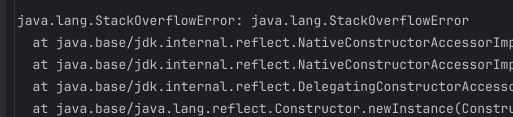
\includegraphics[width=0.8\textwidth]{images/stackOverFlow.jpg}
    \end{figure}

    \subsection{Impacto}

\section{Pruebas y Resultados}

  \subsection{Pruebas}
  Se realizaron mediciones de tiempo para las funciones \texttt{confBiasUpdate} y \texttt{rho} (versiones secuenciales) y sus contrapartes paralelas (\texttt{confBiasUpdatePar} y \texttt{rhoPar}) utilizando tamaños de entrada (\texttt{n}) que son potencias de 2. La aceleración fue calculada como:
  \[
  \text{Aceleración} = \frac{\text{Tiempo secuencial}}{\text{Tiempo paralelo}}.
  \]
  \begin{table}[H]
  \centering
  \begin{tabular}{@{}cccc@{}}
  \toprule
  \textbf{n} & \textbf{Tiempo Par (ms)} & \textbf{Tiempo Seq (ms)} & \textbf{Aceleración (t1/t2)} \\ \midrule
  4 & 0.007 & 0.0938 & 0.0745.. \\
  8 & 0.0108 & 0.083 & 0.1313.. \\
  16 & 0.0196 & 0.1311 & 0.1502.. \\
  32 & 0.0413 & 0.1495 & 0.2769.. \\
  64 & 0.1662 & 0.2811 & 0.59104.. \\
  128 & 0.6421 & 0.5729 & 1.1207.. \\
  256 & 1.8277 & 1.9542 & 1.2324.. \\
  512 & 6.7979 & 4.4917 & 1.5134.. \\

  \bottomrule
  \end{tabular}
  \caption{Comparación de tiempos y aceleración entre confBiasUpdate y confBiasUpdatePar para $2^8$ datos.}
  \label{tab:comparison}
  \end{table}
  \begin{table}[H]
  \centering
  \begin{tabular}{@{}cccc@{}}
    \toprule
    \textbf{n} & \textbf{Tiempo Par (ms)} & \textbf{Tiempo Seq (ms)} & \textbf{Aceleración (t1/t2)} \\ \midrule
    4 & 0.1055 & 0.3369 & 0.31315 \\ 
    8 & 0.0395 & 0.2206 & 0.17906 \\ 
    16 & 0.0461 & 0.1751 & 0.26328 \\ 
    32 & 0.0310 & 0.3096 & 0.10013 \\ 
    64 & 0.0360 & 0.2015 & 0.17866 \\ 
    128 & 0.0486 & 0.2894 & 0.16793 \\ 
    256 & 0.0561 & 0.3393 & 0.16534 \\ 
    512 & 0.0843 & 0.3753 & 0.22462 \\ 
    1024 & 0.1703 & 0.4148 & 0.41056 \\ 
    2048 & 0.2911 & 0.6719 & 0.43325 \\ 
    4096 & 0.7161 & 0.9556 & 0.74937 \\ 
    8192 & 1.0138 & 0.9200 & 1.09873 \\
    16384 & 1.6791 & 1.0050 & 1.15964 \\
    \bottomrule
  \end{tabular}
  \caption{Comparación de tiempos y aceleración entre rho y rhoPar para $2^14$ datos.}
  \label{tab:comparison}
  \end{table}

  \subsection{Resultados}
    \subsubsection{Para \texttt{confBiasUpdate} y \texttt{confBiasUpdatePar}}
    \begin{itemize}
        \item En tamaños pequeños ($n = 4, 8, 16, 32, 64$), la aceleración es menor que 1 ($t_1/t_2 < 1$), lo que indica que la versión paralela es más lenta debido al \textit{overhead} de paralelización.
        \item A partir de $n = 128$, la aceleración supera 1, alcanzando un valor máximo de 1.5134 para $n = 512$, lo que demuestra que la paralelización es efectiva para los tamaños grandes.
    \end{itemize}

    \subsubsection{Para \texttt{rho} y \texttt{rhoPar}}
    \begin{itemize}
        \item Para valores pequeños de $n$ ($n = 4$ a $n = 2048$), la aceleración es bastante menor que 1, lo que indica que la versión paralela tiene un costo adicional significativo.
        \item A partir de $n = 8192$, la aceleración supera 1, lo que conlleva a obtener una mejora significativa.
    \end{itemize}

  \subsection{Análisis de Aceleración}
  La eficiencia de la paralelización depende del tamaño de la entrada (\texttt{n}):

  \begin{itemize}
      \item \textbf{Para \texttt{confBiasUpdatePar}:}
      \begin{itemize}
          \item La aceleración mejora proporcionalmente a medida que $n$ aumenta.
          \item En tamaños pequeños, el costo de gestionar \textit{threads (hilos)} supera los beneficios.
          \item En tamaños grandes ($n \geq 128$), el tiempo paralelo es significativamente mejor, logrando más de 1.5 veces la eficiencia de la versión secuencial para el caso de $n = 512$.
      \end{itemize}

      \item \textbf{Para \texttt{rhoPar}:}
      \begin{itemize}
          \item La aceleración es mucho más dependiente del tamaño de $n$. Incluso para tamaños moderados ($n = 128$ a $n = 2048$), el \textit{overhead} sigue siendo considerable.
          \item El umbral para que la paralelización sea eficiente es mucho mayor, con resultados favorables solo a partir de $n = 8192$.
      \end{itemize}
  \end{itemize}

\section{Conclusiones}
\begin{itemize}
    \item \textbf{\textit{Overhead} inicial:} Para tamaños pequeños de $n$, el \textit{overhead} de paralelización (coordinación de tareas, comunicación entre hilos, etc.) reduce el beneficio de usar la versión paralela, haciendo que sea más lenta que la versión secuencial.
    \item \textbf{Escalabilidad:} A partir de $n = 128$ en \texttt{confBiasUpdatePar} y $n = 8192$ en \texttt{rhoPar}, la paralelización comienza a ser eficiente, lo que muestra que estas funciones están mejor diseñadas para escenarios de mayor tamaño.
    \item \textbf{Umbral de eficiencia:}
    \begin{itemize}
        \item Para \texttt{confBiasUpdatePar}, la paralelización es útil a partir de $n = 128$.
        \item Para \texttt{rhoPar}, es necesario trabajar con tamaños $n \geq 8192$ para que sea rentable.
    \end{itemize}
    \item \textbf{Recomendaciones:}
    \begin{itemize}
        \item Usar \textbf{versiones secuenciales} para tamaños pequeños y medianos ($n < 128$).
        \item Usar \textbf{versiones paralelas} solo cuando $n$ sea lo suficientemente grande para justificar el \textit{overhead}, siendo más efectiva en \texttt{confBiasUpdatePar} que en \texttt{rhoPar}.
    \end{itemize}
\end{itemize}

\end{document}